%- Section 1 ----------------------------------------------------------------
\label{seq:EvolutionaryStrategies}
Folgende Information entstammen im Wesentlichen aus \cite{kost2003optimierung},\cite{bronstejn2012taschenbuch}\ sowie \cite{Hansen:1} und sind auf den folgenden Seiten lediglich zusammengefasst und neu arrangiert um eine Einarbeitung in die Thematik zu ermöglichen.\\
%------------------------------------------------------------------
\subsection{Evolutionsstrategien - Grundlagen }
%
Nach dem Vorbild natürlicher Evolution entworfene stochastische Optimierungsverfahren werden Evolutionsstrategie bezeichnet. Sie verwenden die Prinzipien der Mutation, Rekombination und Selektion analog zu der nat. Evolution. Der Grundlegende Ablauf dieser Strategien zeigt die Abbildung~\ref{es_flowchart}\\
Wie in der Natur auch werden Nachkommen aus der Menge der verfügbaren Eltern gebildet. Dabei bezeichnet im Folgenden:
%
\begin{itemize}
	\item $\mu$ die Anzahl der Eltern (=> Größe der Population)
	\item $\lambda$\footnote{Anmerkung: Die Verwendung des Symbols $\lambda$ ist in diesem Kontext nicht eindeutig. Im Rahmen dieser Arbeit steht dieses Symbol auch für die Wellenlänge. In diesem Abschnitt wird jedoch weiterhin $\lambda$ verwendet um die gleiche Nomenklatur wie bei dieser Thematik üblich zu verwenden.} die Anzahl der Eltern die bei Rekombination neue Kinder erzeugt; Die Anzahl der erzeugten Nachkommen einer neuen Generation
	\item $\mathbf{x}_p$ Elternpunkt (Parent)
	\item $\mathbf{x}_c$ Nachkomme einer Generation (Child)
	\item $X_p^1$ Die Menge aller Eltern der ersten Generation $X_p = \{\mathbf{x}_{p_1}^1,..,\mathbf{x}_{p_\mu}^1\}$
	\item $X_p^k$ Die Menge aller Eltern der k-ten Generation $X_p = \{\mathbf{x}_{p_1}^k,..,\mathbf{x}_{p_\mu}^k\}$
\end{itemize}
%
Wir wollen nun in Abbildung~\ref{fig:es_flowchart} einen Blick auf den prinzipiellen Ablauf dieses Algorithmus werfen und anschließend auf die Details eingehen.
%
%------------------------------------------------------------------------------
%------------------------------------------------------------------------------
%------------------------------------------------------------------------------
\begin{figure}[h]
	\begin{center}
		\caption[Ablauf Evolutionsstrategie]{Der Prinzipielle Ablauf des $(\lambda,\mu)$-Evolutionsalgorithmus.}
		\label{fig:es_flowchart}
		\vspace{0.5cm}
		\begin{tikzpicture}[auto]
		\scriptsize
			\tikzstyle{decision} = [diamond, draw=black, thick, fill=black!20, text width=5em, text badly centered, inner sep=1pt]
%			
			\tikzstyle{block} = [rectangle, draw=black, thick, fill=gray!20, text width=15em, text centered, rounded corners, minimum height=4em]
%	
			\tikzstyle{line} = [draw, thick, -latex',shorten >=1pt];
			\tikzstyle{commentline} = [draw, dashed, green!50,-latex',shorten >=1pt];
%	
			\tikzstyle{cloud} = [ dotted, draw=green!50, thick, ellipse,,fill=green!20, minimum height=2em, text width= 10em, text badly centered];
%	
			\matrix [column sep=5mm,row sep=7mm]
			{
				% row 1
				& \node [block] (start) { Start }; & \\
				% row 2
				&\node [block] (init) {Erstelle Startpopulation $X_p^1$ bestehend aus $\mu$-Individuen }; & 
				\node [cloud] (comment1) {Initialisierung, mit Zufallswerten}; \\
				% row 4
				& \node [block] (identify) {Erzeuge eine Menge von $\lambda$ Nachkommen $X_c^k$ aus der aktuellen Elterngeneration $X_p^k$ durch Rekombination \&\&, || Mutation}; & \\
				% row 5
				\node [block] (update) {Nächste Stufe der Evolution; k++}; &
				\node [block] (evaluate) {Durch Selektion die besten $\mu$ Nachkommen für die Generation $X_p^{k+1}$ auswählen}; & \\
				% row 6
				& \node [decision] (decide) {$\Delta \geq \Delta_{min}$}; & 
				\node [cloud] (criteria) {Abbruchkriterium; Muss geeignet gewählt werden, bspw. max. Anzahl der Generationen oder Erreichen des Optimums};\\
				% row 7
				& \node [block] (stop) {Ende}; & \\
			};
% Arrows
			\tikzstyle{every path}=[line]
			\path (init) -- (identify);
			\path (identify) -- (evaluate);
			\path (evaluate) -- (decide);
			\path (update) |- (identify);
			\path (decide) -| node [near start] {Ja} (update);
			\path (decide) -- node [midway] {Nein} (stop);
			\path (start) -- (init);
			
			\tikzstyle{every path}=[commentline]
			\path (criteria) -- (decide);
			\path (comment1) -- (init);
			
		\end{tikzpicture}
	\end{center}
\end{figure}
%------------------------------------------------------------------
\begin{figure} [ht!]
\centering
         \caption[Konzept direkter Optimierung mittels CMA-ES]{Die Abbildung zeigt sechs Lösungsschritte des CMA-ES-Verfahrens. Eingangs wird eine Population mit einer Gauß-Verteilung generiert. Diese bewegt sich von Generation näher an das globale Optimum. Die gestrichelte Linie zeigt dabei eine Isolinie der Wahrscheinlichkeitsdichte. Wir befinden uns auf einem 2D-Problem, somit wird das vorankommen der Population über zwei $\sigma$'s gesteuert. Dadurch kommt die Ellipse zu Stande. Die Linie bedeutet nicht, dass nur in diesem Bereich Nachkommen erzeugt werden, siehe z.B. Generation 4. Je nach Beschaffenheit des Problems und nach Nähe zum Optimum werden die steuernden $\sigma$'s kleiner. }
         \label{fig:conecpt_cma.es}
         \vspace{0.5cm}
         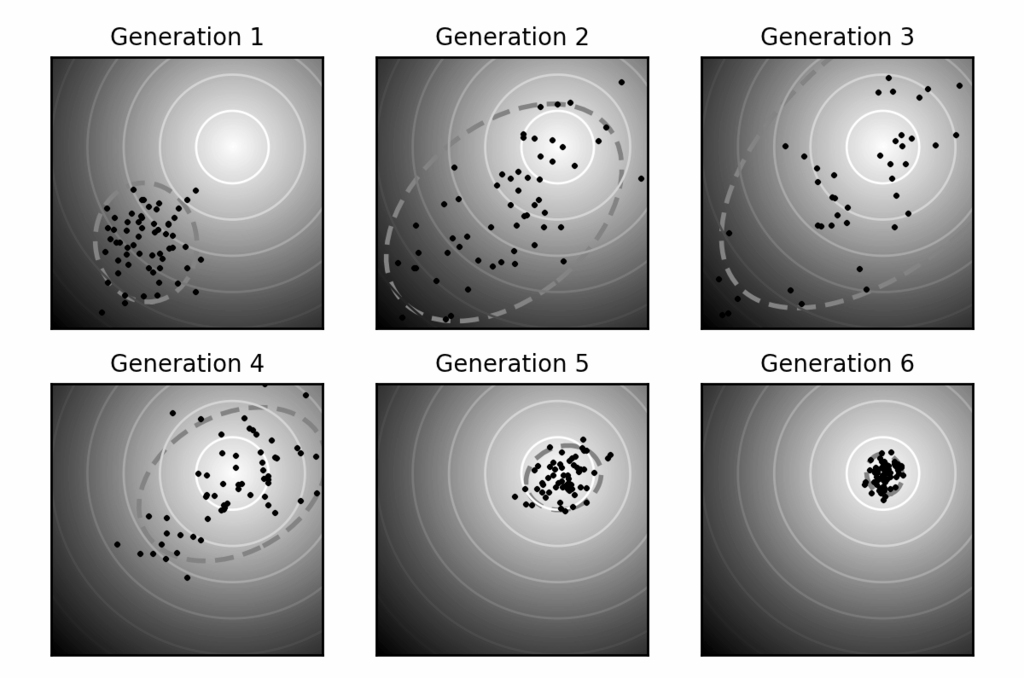
\includegraphics[width=\textwidth]{img/CMA-ES_algorithm.png}
%      
\end{figure}
%
%------------------------------------------------------------------
\subsubsection[Mutation]{Mutation}
Ein Nachkomme $\mathbf{x}_C$ wird aus seinem Elternteil $\mathbf{x}_P$ und einer zufälligen Variation $\mathbf{d}$ gebildet.
\begin{equation} \label{eq:Mutation_Child}
	\mathbf{x}_c = \mathbf{x}_P + \mathbf{d}
\end{equation}
Dabei ist $\mathbf{d}$ ein bei jeder Mutation neu zu bestimmender $(0,\sigma^2)-normalverteilte$ Zufallszahl $Z(0,\sigma^2)$:
\begin{equation}\label{eq:wavenumber_trilateration_model2}
\mathbf{d}=
\left(
	\begin{array}{c}
		d_1 \\
		\vdots\\
		d_n 
	\end{array}
\right)
=
\left(
	\begin{array}{c}
		Z(0,\sigma_1^2) \\
		\vdots\\
		Z(0,\sigma_n^2) 
	\end{array}
\right)
=
\left(
	\begin{array}{c}
		Z(0,1) \sigma_1 \\
		\vdots\\
		Z(0,1) \sigma_n 
	\end{array}
\right)
\end{equation}
%
Die Normalverteilung der Variation ist nützlich, da kleine Änderungen wahrscheinlicher sind als große. Die maximale Größe der Variation wird durch die Standardabweichung $\sigma_i$ bestimmt. Sie steuert somit die Schrittweite von Generation zu Generation.
%
%------------------------------------------------------------------
\subsubsection[Rekombination]{Rekombination}
Durch Rekombination zweier oder mehr Eltern aus der Menge aller $\mu$-Eltern $X_{\varrho} \subset X_E$. Die Wahl der Eltern sollte zufällig erfolgen um Inzuchtprobleme zu verhindern.\\
Zwei Arten der Rekombination sind denkbar:\\

Die \textit{intermediär Rekombination} erstellt einen Nachkommen durch das gewichtete Mittel von $\varrho$ Eltern.
%
\begin{equation}
\mathbf{x}_c = \Sigma^\varrho_{i=1} \alpha_i\mathbf{x}_{p_i},\\ \Sigma^\varrho_{i=1} \alpha_i = 1,\\ 2\leq\varrho\leq\mu
\end{equation} 
%
Bei der \textit{diskreten Rekombination} vom $\varrho$-Eltern wird die \textit{i}-te Komponente $x_{ic}$ eines Nachkommen $\mathbf{x}_c$ mit der \textit{i}-te Komponente eines zufällig gewählten Elternpunktes gleichgesetzt.
%
\begin{equation}
\mathbf{x}_{ic} = \mathbf{x}_{ip_j},\\ j\in\{1,...,\varrho\},\\i=1,...,n
\end{equation} 
%
%- Section .4 -----------------------------------------------------------------
\subsubsection[Selektion]{Selektion}
Die durch Rekombination und/oder Mutation erzeugten Nachkommen werden in dem Schritt Ausgewählt um einen Evolutionsfortschritt zu erreichen. Dies erfolgt anhand des Vergleichs mit dem Zielfunktionswert $f(\mathbf{x})$. Das beste Individuum oder die besten werden für die nachfolgende Generation ausgewählt. Dabei gibt es Strategien bei denen nur die Nachkommen an der Auswahl beteiligt sind und welche bei denen Eltern und Kinder teilnehmen.

%- Section .5 -----------------------------------------------------------------
\subsubsection{Evolutionsalgorithmus}
%
Der eigentliche Evolutionsalgorithmus ist in Abbildung~\ref{fig:es_flowchart} dargestellt. Er enthält im wesentlichen die in den vorherigen Abschnitten beschriebenen Schritte. Der prinzipielle Ablauf ist für alle Evolutionsalgorithmen gleich. Eine Unterscheidung der Verfahren kann durch verschiedene Parameter beschrieben werden. Wesentlich dabei sind die Populationsgröße $\mu$, die Anzahl an der Rekombination beteiligten Eltern $\varrho$, die gewählte Selektionsstrategie sowie die Anzahl der Nachkommen $\lambda$. Im Folgenden sind zuerst einige Beispiele für die Nomenklatur der Selektionsstrategie aufgeführt, die im Anschluss genauer beschrieben werden.\\
Für Strategien die nur auf Mutation für die Erzeugung von Nachkommen setzten sind folgende Nomenklaturen gebräuchlich:
\begin{itemize}
\item $(\mu+\lambda)$ Elternelemente werden in der Selektion berücksichtigt
\item $(\mu,\lambda)$ Ausschließlich Nachkommen nehmen an der Selektion teil
\end{itemize}
%
Die Strategien werden Plus- bzw. Komma-Strategie genannt. bei der Plus-Strategie wird zusätzlich noch ein gewichtungsfaktor eingeführt, der das "altern" der Elterngeneration darstellt. Dieser Mechanismus soll verhindern, dass die Eltern, nach einer gewissen Anzahl an Generationen, nicht mehr berücksichtigt werden.\\
Wird die Rekombination eingesetzt kann auch die Anzahl der beteiligten Elternelemente angegeben werden:
\begin{itemize}
\item $({\mu}/{\varrho}+\lambda)$ \& $({\mu}/{\varrho},\lambda)$ Angabe der Anzahl beteiligter Eltern bei der Rekombination.
\end{itemize}
%
Mithilfe der hier beschrieben Klassifikationen werden die Algorithmen im Folgenden stets angegeben.\\

In Abbildung~\ref{fig:es_flowchart} wird der Ablauf einer Optimierung mit evolutionären Verfahren dargestellt. Es wird die Komma-Strategie gezeigt, ein Struktogramm der Plus-, oder anderer Strategien ist nicht gezeigt. Die Unterschiede würden sich in dem Punkt Rekombination zeigen.
%
%------------------------------------------------------------------------------
%- Section .6 -----------------------------------------------------------------
\subsection{Strategien mit mehreren Populationen}
Es ist möglich die Strategien auf die Ebene von Populationen zu erweitern. Das bedeutet, man lässt ganze Populationen miteinander in Wettstreit treten und nur diejenige überleben, die die besten Ergebnisse liefern. Das mündet in einem zweistufigen Evolutionsprozess. Man kann die Notation um diesen Umstand erweitern und erhält so:
$$
[\mu_2/\varrho_2,^{+}\lambda_2(\mu_1/\varrho_1,^{+}\lambda_1)]
$$
Sprich aus $\mu_2$-Elternpopulationen werden durch Rekombination mit jeweils $\varrho_2$ Populationen, $\lambda_2$ Nachkommenpopulationen generiert. Innerhalb der Populationen erfolgt die Optimierung anhand einer $({\mu_1}/{\varrho_1}+\lambda_1)$ oder $({\mu_1}/{\varrho_1},\lambda_1)$-Strategie. Nun kann nach einer bestimmten Zahl von Generationen die besten Populationen für die nächste Generation ausgewählt werden. Auch hier stehen verschiedene Auswahlkriterien zur Verfügung. Man kann z.B. die Population anhand des Zielfunktionswert des besten Individuums wählen oder den Mittelwert über alle Individuen wählen.
%
%- Section .7 -----------------------------------------------------------------
\subsection{Optimierungsräume}
\lipsum[1]
%
\subsubsection{Kontinuierliche Optimierung}
%
\lipsum[1]
%
\subsubsection{Diskrete Optimierung}
%
\lipsum[1]
%
\subsubsection{Gemischte Optimierung}
%
\lipsum[1]
%
%- Section .8 -----------------------------------------------------------------

